\documentclass{beamer}

\usepackage{bussproofs}
\usepackage{stmaryrd}
\usepackage[utf8]{inputenc}
\usepackage{pgfpages}
\usepackage{mathtools}
\usepackage{array}
\usepackage{drs}
\input{qobitree}
\usepackage{listings}


\setbeamertemplate{navigation symbols}{}
\setbeamertemplate{footline}
  {\hfill {\normalsize \insertframenumber{}/\inserttotalframenumber{}}}
\hypersetup{pdfstartview={Fit}}

\AtBeginSection[]
{
\begin{frame}{Outline}
  \tableofcontents[currentsection]
\end{frame}
}

\newcommand{\hsbind}{\mathbin{\gg\!=}}
\newcommand{\apl}{\mathbin{\ll\!\!\cdot}}
\newcommand{\apr}{\mathbin{\cdot\!\!\gg}}
\newcommand{\aplr}{\mathbin{\ll\!\!\cdot\!\!\gg}}
\newcommand{\cons}{\mathbin{::}}
\newcommand{\cat}{\mathbin{+\mkern-10mu+}}

\newcommand{\abs}[1]{\textsc{#1}}
\newcommand{\obj}[1]{\textbf{#1}}
\newcommand{\sem}[1]{\llbracket #1 \rrbracket}
\newcommand{\lex}[2]{\sem{\abs{#1}} &:= #2}

\newcommand{\semdom}[1]{\textbf{#1}}

\newcommand{\dand}{\mathbin{\overline{\land}}}
\newcommand{\dnot}{\mathop{\overline{\lnot}}}
\newcommand{\dor}{\mathop{\overline{\lor}}}
\newcommand{\dimpl}{\mathbin{\overline{\to}}}
\newcommand{\dexists}{\mathop{\overline{\exists}}}
\newcommand{\dforall}{\mathop{\overline{\forall}}}

\newcommand{\limp}{\mathbin{{-}\mkern-3.5mu{\circ}}}

\newcommand{\llbparenthesis}{\vcenter{\hbox{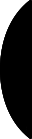
\includegraphics{symbols/llbparenthesis.png}}}}
\newcommand{\rrbparenthesis}{\vcenter{\hbox{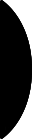
\includegraphics{symbols/rrbparenthesis.png}}}}
\newcommand{\lban}{\llparenthesis \,}
\newcommand{\rban}{\, \rrparenthesis}
\newcommand{\lbban}{\llbparenthesis \,}
\newcommand{\rbban}{\, \rrbparenthesis}
\newcommand{\banana}[1]{\lban #1 \rban}
\newcommand{\bbanana}[1]{\lbban #1 \rbban}
\newcommand{\cherry}{\rotatebox[origin=c]{270}{$\limp$}}

\newcommand{\lam}[2]{\lambda #1.\, #2}
\newcommand{\ap}[2]{#1\,#2}
\newcommand{\app}[3]{\ap{\ap{#1}{#2}}{#3}}
\newcommand{\appp}[4]{\ap{\ap{\ap{#1}{#2}}{#3}}{#4}}
\newcommand{\op}[1]{\mathtt{#1}}
\newcommand{\onto}[1]{#1 \mathalpha{:\,}}
\newcommand{\typedop}[3]{\op{#1} : #2 \rightarrowtail #3}
\newcommand{\typedopg}[3]{#1 : #2 \rightarrowtail #3}
\newcommand{\row}[2]{\{ #1 \mathrel{|} #2 \}}

\newcommand{\CC}{\mathcal{C}}
\newcommand{\FF}{\mathcal{F}}
\newcommand{\GG}{\mathcal{G}}
\newcommand{\XX}{\mathcal{X}}
\newcommand{\EE}{\mathcal{E}}
\newcommand{\TT}{\mathcal{T}}
\newcommand{\PP}{\mathcal{P}}

\newcommand{\FV}{\operatorname{FV}}

\newcommand{\subst}[3]{#1[#2 \coloneqq #3]}

\newcommand{\syntclos}[1]{\mathbin{[#1]}}





\newcommand{\cibanana}{\banana{(\onto{\op{op}_i} M_i)_{i \in I},\ \onto{\eta} M_\eta}}
\newcommand{\cdbanana}{\banana{\onto{\op{op}_1} M_1,\ \dots,\ \onto{\op{op}_n} M_n,\ \onto{\eta} M_\eta}}

\newcommand{\cibbanana}{\bbanana{(\onto{\op{op}_i} M_i)_{i \in I},\ \onto{\eta} M_\eta}}

\newcommand{\TODO}[1]{\textcolor{red}{\textbf{TODO}: #1}}

\newcommand{\relR}{\mathbin{R}}

\newcommand{\swap}{\mathbin{\textbf{swap}}}

\newcommand{\tto}{\twoheadrightarrow}

\mathchardef\mhyphen="2D

\newcommand{\pair}[2]{\left<#1, #2\right>}
\newcommand{\inl}{\operatorname{inl}}
\newcommand{\inr}{\operatorname{inr}}
\newcommand{\case}[5]{\text{\textbf{case} $#1$ \textbf{of} $\{ \ap{\inl}{#2} \to #3;\ \ap{\inr}{#4} \to #5 \}$}}
\newcommand{\absurd}[1]{\text{\textbf{case} $#1$ \textbf{of} \{\,\}}}

\newcommand{\true}{\textbf{T}}
\newcommand{\false}{\textbf{F}}
\newcommand{\ifte}[3]{\text{\textbf{if} $#1$ \textbf{then} $#2$ \textbf{else} $#3$}}


% Examples
\newcommand{\expr}[1]{\textsc{#1}}
\newcommand{\sume}{\expr{sum}}
\newcommand{\prode}{\expr{prod}}
\newcommand{\lite}{\expr{lit}}
\newcommand{\dive}{\expr{div}}
\newcommand{\trye}{\expr{try}}
\newcommand{\lete}{\expr{let}}
\newcommand{\vare}{\expr{var}}
\newcommand{\sumecn}[2]{\app{\sume}{#1}{#2}}
\newcommand{\prodecn}[2]{\app{\prode}{#1}{#2}}
\newcommand{\litecn}[1]{\ap{\lite}{#1}}
\newcommand{\divecn}[2]{\app{\dive}{#1}{#2}}
\newcommand{\tryecn}[2]{\app{\trye}{#1}{#2}}
\newcommand{\letecn}[3]{\appp{\lete}{\bar{#1}}{#2}{#3}}
\newcommand{\varecn}[1]{\ap{\vare}{#1}}

\newcommand{\paren}[1]{(#1)}

\newcommand{\sumec}[2]{\paren{\sumecn{#1}{#2}}}
\newcommand{\prodec}[2]{\paren{\prodecn{#1}{#2}}}
\newcommand{\litec}[1]{\paren{\litecn{#1}}}
\newcommand{\divec}[2]{\paren{\divecn{#1}{#2}}}
\newcommand{\tryec}[2]{\paren{\tryecn{#1}{#2}}}
\newcommand{\letec}[3]{\paren{\letecn{#1}{#2}{#3}}}
\newcommand{\varec}[1]{\paren{\varecn{\bar{#1}}}}


\newcommand{\NN}{\mathbb{N}}
\newcommand{\dbze}{\frac{\cdot}{0}}
\newcommand{\dbzelong}{\operatorname{DivisionByZero}}


\newcommand{\reseto}{\mathtt{reset0}}
\newcommand{\shifto}{\mathtt{shift0}}
\newcommand{\resetobanana}{\banana{\onto{\op{shift0}}{(\lam{c k}{\ap{c}{k}})}}}
\newcommand{\from}{\leftarrow}

\newcommand*{\twoheadleftrightarrow}{%
  \twoheadleftarrow
  \mathrel{\mkern-15mu}%
  \twoheadrightarrow
}

\newcommand{\ffrom}{\twoheadleftarrow}
\newcommand{\ttoffrom}{\twoheadleftrightarrow}


\newcommand{\reset}{\mathtt{reset}}
\newcommand{\shift}{\mathtt{shift}}

\newcommand{\semo}[1]{\sem{#1}_0}


\newcommand{\demph}[1]{\textbf{#1}}



\newcommand{\set}{\texttt{set}}
\newcommand{\get}{\texttt{get}}
\newcommand{\sel}{\texttt{sel}}
\newcommand{\boxop}{\texttt{BOX}}
\newcommand{\oboxop}{\texttt{BOX'}}
\newcommand{\scope}{\texttt{scope}}
\newcommand{\siop}{\texttt{SI}}


\title{DRT as a Programming Language}
\author{Jirka Maršík}
\date{Feb 4, 2016}
\institute{INRIA/LORIA}


\begin{document}

\begin{frame}
  \maketitle
\end{frame}

\section{$\lambda$-calculus with State}

\begin{frame}{$\lambda_\set$ --- Syntax}
  \begin{align*}
  V ::= &\ \lam{x}{M} \\
   | \, &\ x \\
  M, N ::= &\ V \\
   | \, &\ (\ap{M}{N}) \\
   | \, &\ (\ap{\set}{M}) \\
   | \, &\ \get
  \end{align*}
  \begin{itemize}
  \item term/value distinction
  \item new operators $\set$ and $\get$
  \end{itemize}
\end{frame}

\begin{frame}{$\lambda_\set$ --- Contexts}
  \begin{align*}
  C ::= &\ [] \\
  | \, &\ (\ap{C}{M}) \\
  | \, &\ (\ap{V}{C}) \\
  | \, &\ (\ap{\set}{C})
  \end{align*}
  $$
  C[M] \, = \, C[[] := M]
  $$
  \begin{itemize}
  \item $M = C[N]$
    \begin{itemize}
    \item $N$ is the next subterm of $M$ to be evaluated
    \end{itemize}
  \end{itemize}
\end{frame}

\begin{frame}{$\lambda_\set$ --- Operational Semantics}
  \begin{center}
   \begin{tabular}{>{$}r<{$} >{$}c<{$} >{$}l<{$}}
     (C[{\color<2->{blue}{\ap{(\lam{x}{M})}{V}}}], {\color<3->{red}{\sigma}})
   & \to_\beta
   & (C[{\color<2->{blue}{\subst{M}{x}{V}}}], {\color<3->{red}{\sigma}}) \\
     (C[{\color<2->{blue}{\ap{\set}{V}}}], {\color<3->{red}{\sigma}})
   & \to_\set
   & (C[{\color<2->{blue}{V}}], {\color<3->{red}{V}}) \\
     (C[{\color<2->{blue}{\get}}], {\color<3->{red}{\sigma}})
   & \to_\get
   & (C[{\color<2->{blue}{\sigma}}], {\color<3->{red}{\sigma}})
  \end{tabular}
  \end{center}
\end{frame}

\begin{frame}{$\lambda_\set$ --- Semantics, DRT Style}
  \begin{block}{$\set$}
   \vspace{4mm}
   \begin{tabular}{ll}
    \textbf{Triggering configuration in $C[M]$:} & $(\ap{\set}{V})$ \\
    \textbf{Set:} & the state to the value $V$ \\
    \textbf{Substitute in $M$:} & $V$ for $(\ap{\set}{V})$
  \end{tabular}
  \end{block}
  \pause
  \vspace{1cm}
  \begin{block}{\get}
   \vspace{4mm}
   \begin{tabular}{ll}
    \textbf{Triggering configuration in $C[M]$:} & $\get$ \\
    \textbf{Get:} & the current state $\sigma$ \\
    \textbf{Substitute in $M$:} & $\sigma$ for $\get$
  \end{tabular}
  \end{block}
\end{frame}

\begin{frame}[fragile]{$\lambda_\set$ --- Example}
  \begin{lstlisting}
let t = set (fun x y -> x) in
let f = set (fun x y -> y) in
get (fun f x -> f x) (fun f x -> x)
  \end{lstlisting}
  \vfill
  $$
  \ap{(\lam{{\color{red}{t}}}{\ap{(\lam{{\color{blue}{f}}}{\app{\get}{(\lam{f x}{\ap{f}{x}})}{(\lam{f x}{x})}})}{{\color{blue}{(\ap{\set}{(\lam{x y}{y})})}}}})}{{\color{red}{(\ap{\set}{(\lam{x y}{x})})}}}
  $$
\end{frame}


\section{Discourse Representation Theory}

\begin{frame}{DRS Construction Algorithm}
  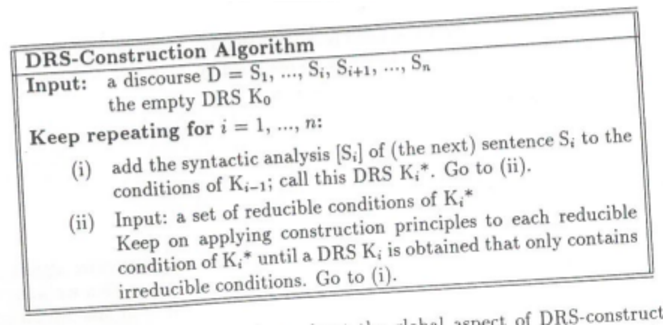
\includegraphics[width=\textwidth]{cr-algo}
\end{frame}

\begin{frame}{Example DRS Derivations}
 \begin{center}
  \begin{tabular}{rcl}
   \drs{ \quad }{
     A boy sleeps
   }
 & \pause $\to$
 & \drs{ x }{
     $\semdom{boy}(x)$ \\
     $x$ sleeps
   } \\ \\ \\
   \pause \drs{ x }{
     $\semdom{boy}(x)$ \\
     $x$ sleeps \\
     He dreams
   }
 & \pause $\to$
 & \drs{ x, y }{
     $\semdom{boy}(x)$ \\
     $x$ sleeps \\
     $y = x$ \\
     $y$ dreams
   }
  \end{tabular}
 \end{center}
\end{frame}

\begin{frame}{DRT --- Terms and Values}
  \begin{itemize}
  \item values: semantic objects (discourse referents)
  \item terms: syntactic objects (parse trees)
    \begin{itemize}
    \item May contain traces of semantic objects.
    \end{itemize}
  \end{itemize}

  \begin{columns}
    \begin{column}{0.5\textwidth}
      \leaf{A}
      \branch{1}{DET}
      \leaf{boy}
      \branch{1}{N}
      \branch{2}{NP}
      \leaf{sleeps}
      \branch{1}{V}
      \branch{1}{VP}
      \branch{1}{VP'}
      \branch{2}{S}
      \tree
    \end{column}
    \begin{column}{0.5\textwidth}
      \leaf{$x$}
      \leaf{sleeps}
      \branch{1}{V}
      \branch{1}{VP}
      \branch{1}{VP'}
      \branch{2}{S}
      \tree
    \end{column}
  \end{columns}
\end{frame}

\begin{frame}{DRT --- Contexts}
  We can reduce\ldots
  \begin{itemize}
  \item within any sub-tree
  \item within any (uninterpreted) condition
  \item within any DRS 
  \end{itemize}
  \pause
  provided that
  \begin{itemize}
    \item there is no other redex containing our redex.
  \end{itemize}
\end{frame}

\begin{frame}{DRT --- Contexts, Formally}
  \begin{align*}
  C ::= &\ \drs{ $x_1$, \ldots, $x_n$ }
               { $\gamma_1$ \\ \ldots \\ $C_\gamma$ \\ \ldots
                 \\ $\gamma_m$}
         \quad | \quad \drs{ $x_1$, \ldots, $x_n$ }
               { $\gamma_1$ \\ \ldots \\ $\lnot C$ \\ \ldots \\ $\gamma_m$ } \\ \\
  C_\gamma ::= &\ []\ |\ \leaf{$C_\gamma$} \leaf{VP} \branch{2}{S} \tree
                    \ |\ \leaf{NP} \leaf{$C_\gamma$} \branch{2}{S} \tree
                    \ |\ \leaf{$C_\gamma$} \leaf{NP} \branch{2}{VP} \tree
                    \ |\ \leaf{V} \leaf{$C_\gamma$} \branch{2}{VP} \tree \ |\ \ldots
  \end{align*}
\end{frame}

\begin{frame}{DRT Construction Rules}
  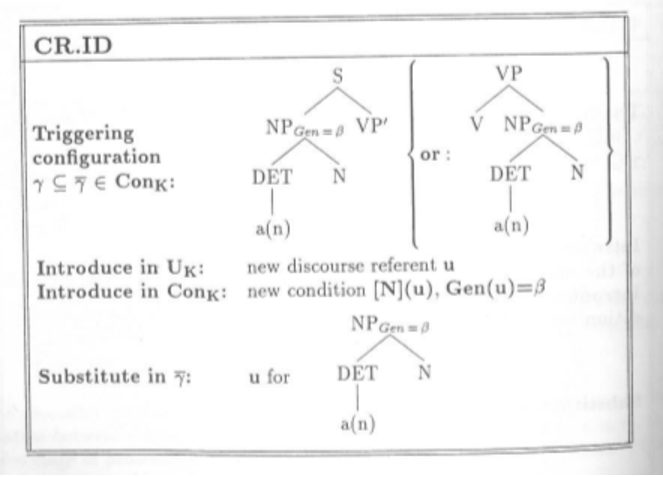
\includegraphics[width=\textwidth]{cr-id}
\end{frame}

\begin{frame}{DRT Construction Rules}
  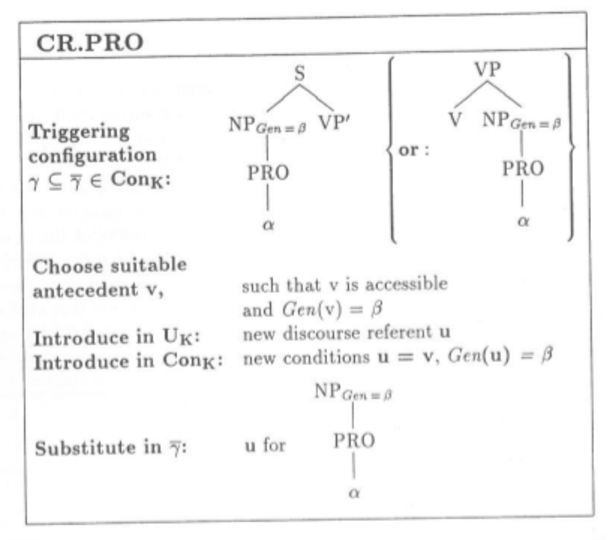
\includegraphics[height=\textheight]{cr-pro}
\end{frame}

\begin{frame}{DRT, Reduction Style}
  $$
  C\left[\ \drs{$x_1$, \ldots, $x_n$}
        {$\gamma_1$ \\
         \ldots \\
         $\left( \leaf{$\alpha$} \branch{1}{PRO} \branch{1}{NP$_{Gen=\beta}$}
         \leaf{VP$'$} \branch{2}{S} \tree \right)$ \\
         \ldots \\
         $\gamma_m$}\ \right]
  \to_{\texttt{CR.PRO}}
  C\left[\ \drs{$x_1$, \ldots, $x_n$, $u$}
        {$\gamma_1$ \\
         \ldots \\
         $u = v$ \\
         $Gen(u) = \beta$ \\
         $\left( \leaf{$u$} \leaf{VP$'$} \branch{2}{S} \tree \right)$ \\
         \ldots \\
         $\gamma_m$}\ \right]
  $$

  where $v$ is a suitable accessible that is accessible and for which
  $Gen(v) = \beta$.
\end{frame}

\begin{frame}[fragile]{DRT, ML Style}
  \begin{lstlisting}
cr_pro (S (NP beta (PRO alpha)) vp) =
  let v = choose (fun v -> gen v = beta) in
  let u = introduce () in
  assert (u = v)
  assert (gen u = beta)
  (S u vp)
  \end{lstlisting}
\end{frame}

\begin{frame}{DRT, Continuation Passing Style}
  \begin{align*}
    \texttt{CR.PRO}_\beta =
    & \app{\op{choose}}{(\lam{v}{Gen(v) = \beta})}{ \only<2->{&} (\lam{v} \\
    & {\ap{\op{introduce}}{ \only<2->{&} (\lam{u} \\
    & {\app{\op{assert}}{(u = v)}{ \only<2->{&} ( \\
    & {\app{\op{assert}}{(Gen(u) = \beta)}{ \only<2->{&} ( \\
    & {\ap{\eta}{u}})}})}})}})}
  \end{align*}
  \pause
  \pause
  \begin{align*}
    \op{choose} &: (\iota \to o) \to \only<4->{&} (\iota \to \FF(\alpha)) \to \FF(\alpha) \\
    \op{introduce} &: \only<4->{&} (\iota \to \FF(\alpha)) \to \FF(\alpha) \\
    \op{assert} &: o \to \only<4->{&} \FF(\alpha) \to \FF(\alpha) \\
    \eta &: \alpha \to \FF(\alpha)
  \end{align*}
\end{frame}

\begin{frame}{DRT, Philippe de Groote Style}
  \begin{align*}
    \FF(\alpha) &= \gamma \to (\alpha \times \gamma \to o) \to o \\
    \FF(1) &\simeq \gamma \to (\gamma \to o) \to o \quad (= \bar{o}) \\
    \op{choose} &= \lam{f k e \phi}{\appp{k}{(\app{\sel}{f}{e})}{e}{\phi}} \\
    \op{introduce} &= \lam{k e \phi}{\exists x. \appp{k}{x}{(x \cons e)}{\phi}} \quad (= \bar{\exists}\ ) \\
    \op{assert} &= \lam{p k e \phi}{p \land (\appp{k}{(p \cons e)}{\phi})} \\
    \eta &= \lam{x e \phi}{\ap{\phi}{(x, e)}}
  \end{align*}
\end{frame}


\section{Smoothing Out the Differences}

\begin{frame}{Simple Example}
  A boy sleeps. He dreams.
  \vfill
  \pause
  In DRT:
  \begin{align*}
    &\ap{\op{introduce}}{&(\lam{x} \\
      {&\app{\op{assert}}{(\semdom{boy}(x))}{&( \\
      {&\app{\op{assert}}{(\semdom{sleeps}(x))}{&( \\
       &\app{\op{choose}}{(\lam{v}{Gen(v) = male})}{&(\lam{v}{ \\
       &\ap{\op{introduce}}{&(\lam{y} \\
      {&\app{\op{assert}}{(y = v)}{&( \\
       &\app{\op{assert}}{(\semdom{dreams}(y))}{&( \\
       &\ap{\eta}{\star})})}})}})})}})}})}
  \end{align*}
\end{frame}

\begin{frame}{Simple Example, Cont'd}
  A boy sleeps. He dreams.
  \vfill
  DRT, result:

  \drs{ $x$, $y$ }
      { $\semdom{boy}(x)$ \\
        $\semdom{sleeps}(x)$ \\
        $y = x$ \\
        $\semdom{dreams}(y)$ }

  \vfill
  \pause
  Static version:
  $$
    \exists x y.\ \semdom{boy}(x) \land \semdom{sleeps}(x) \land y = x
    \land \semdom{dreams}(y)
  $$
\end{frame}

\begin{frame}{Simple Example, in Continuation-based Dynamic Logic}
  A boy sleeps. He dreams.
  \vfill
  In continuation-based dynamic logic:
  \begin{align*}
  \lam{e \phi}{\exists x y.\ &\semdom{boy}(x) \land \semdom{sleeps}(x)
    \land y = x \land \semdom{dreams}(y) \\ & \land
    \ap{\phi}{(\semdom{dreams}(y) \cons (y = x) \cons y \cons \semdom{sleeps}(x)
      \cons \semdom{boy}(x) \cons x \cons e)}}
  \end{align*}
  since
  $$
  \appp{\sel}{(\lam{v}{Gen(v) = male})}{(\semdom{sleeps}(x) \cons
    \semdom{boy}(x) \cons x \cons e)} = x
  $$
  \vfill
  \pause
  Static version:
  $$
    \exists x y.\ \semdom{boy}(x) \land \semdom{sleeps}(x) \land y = x
    \land \semdom{dreams}(y)
  $$
\end{frame}

\begin{frame}{Negation}
  $$
  \bar{\lnot} A = \lam{e \phi}{\lnot(\app{A}{e}{(\lam{e'}{\top})}) \land \ap{\phi}{e}}
  $$
  \pause
  \begin{itemize}
  \item no abstract operations to handle this
  \item let's make new ones
  \end{itemize}
  \pause
  \begin{align*}
  \boxop &: \FF(1) \to \gamma \to o \\
  \boxop &= \lam{A e}{\app{A}{e}{(\lam{e'}{\top})}} \\
  \op{get} &: (\gamma \to \FF(\alpha)) \to \FF(\alpha) \\
  \op{get} &= \lam{k e \phi}{\app{k}{e}{\phi}}
  \end{align*}
\end{frame}

\begin{frame}{Negation, Abstractly}
  Old negation:
  $$
  \bar{\lnot} A = \lam{e \phi}{\lnot(\app{A}{e}{(\lam{e'}{\top})}) \land \ap{\phi}{e}}
  $$
  \pause
  \vfill
  New negation:
  \begin{align*}
    \bar{\lnot} A =\ & \ap{\op{get}}{(\lam{e}{ \\
                    & \app{\op{assert}}{(\lnot(\app{\boxop}{e}{A}))}{( \\
                     & \ap{\eta}{\star})}})}
  \end{align*}
\end{frame}

\begin{frame}{Negation, in DRT}
  \begin{align*}
    \bar{\lnot} A =\ & \ap{\op{get}}{(\lam{e}{ \\
                    & \app{\op{assert}}{(\lnot(\app{\boxop}{e}{A}))}{( \\
                     & \ap{\eta}{\star})}})}
  \end{align*}

  \begin{center}
  Compare with:

  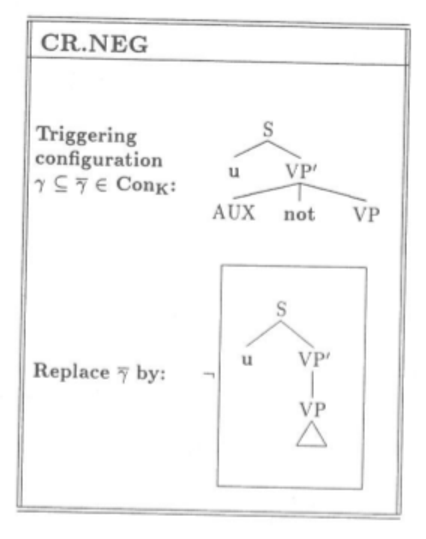
\includegraphics[height=0.5\textheight]{cr-neg}
  \end{center}
\end{frame}

\begin{frame}{Note: $\op{choose}$ is derivable from $\op{get}$ and $\sel$}
  \begin{align*}
    \op{choose} &: (\iota \to o) \to (\iota \to \FF(\alpha)) \to \FF(\alpha) \\
    \op{choose} &= \lam{f k}{\ap{\op{get}}{(\lam{e}{\ap{k}{(\app{\sel}{f}{e})}})}}
  \end{align*}
\end{frame}

\begin{frame}{The DRT Abstract Signature}
  \begin{align*}
    \op{introduce} &: \alt<1>{(\iota \to \FF(\alpha)) \to \FF(\alpha)}
                             {1 \to (\iota \to \FF(\alpha)) \to \FF(\alpha)} \\
    \op{assert} &: \alt<1>{o \to \FF(\alpha) \to \FF(\alpha)}
                          {o \to (1 \to \FF(\alpha)) \to \FF(\alpha)} \\
    \op{get} &: \alt<1>{(\gamma \to \FF(\alpha)) \to \FF(\alpha)}
                       {1 \to (\gamma \to \FF(\alpha)) \to \FF(\alpha)}\\
    \boxop &: \FF(1) \to \gamma \to o
  \end{align*}
  \pause \pause \vfill Or with $\beta_i \rightarrowtail \beta_o = \beta_i
  \to (\beta_o \to \FF(\alpha)) \to \FF(\alpha)$
  \begin{align*}
    \op{introduce} &: 1 \rightarrowtail \iota \\
    \op{assert} &: o \rightarrowtail 1 \\
    \op{get} &: 1 \rightarrowtail \gamma \\
    \boxop &: \FF(1) \to \gamma \to o
  \end{align*}
\end{frame}

\begin{frame}{Note: There is also quantification}
  \begin{align*}
    \sem{NP} &: (\iota \to \gamma \to (\gamma \to o) \to o) \to \gamma \to (\gamma \to o) \to o \\
    &= (\iota \to \FF(1)) \to \FF(1) \\
    &= \GG(\iota) \\
    \GG(\alpha) &= (\alpha \to \FF(1)) \to \FF(1) \\
  \end{align*}
  \pause
  we can distill a signature as well\ldots
  \begin{align*}
    \scope &: ((\iota \to \FF(1)) \to \FF(1)) \to (\iota \to \GG(\FF(1))) \to \GG(\FF(1)) \\
    \scope &= \lam{c k \psi}{\ap{c}{(\lam{x}{\ap{\psi}{(\ap{\siop}{(\ap{k}{x})})}})}} \\
    \siop &: \GG(\FF(1)) \to \FF(1) \\
    \siop &= \lam{f}{\ap{f}{(\lam{x}{x})}}
  \end{align*}
  \pause
  but we will not dwell on it.
\end{frame}



\section{Switching to a Different Model}

\newcommand{\handlerrule}{
 \begin{prooftree}
  \AxiomC{$E = \{\typedopg{\op{op}_i}{\alpha_i}{\beta_i}\}_{i \in I} \uplus E_f$}
  \noLine
  \def\extraVskip{0pt}
  \UnaryInfC{$E' = E'' \uplus E_f$}
  \noLine
  \UnaryInfC{$[\Gamma \vdash M_i : \alpha_i \to (\beta_i \to
    \FF_{E'}(\delta)) \to \FF_{E'}(\delta)]_{i \in I}$}
  \noLine
  \UnaryInfC{$\Gamma \vdash M_\eta : \gamma \to \FF_{E'}(\delta)$}
  \def\extraVskip{2pt}
  \RightLabel{[$\banana{}$]}
  \UnaryInfC{$\Gamma \vdash \cibanana : \FF_{E}(\gamma) \to \FF_{E'}(\delta)$}
 \end{prooftree}}

\begin{frame}{Introducing $\banana{\lambda}$}
 
  \begin{itemize}
  \item terms for computations (operations and $\eta$)
  \end{itemize}
  
   \begin{prooftree}
    \AxiomC{$\Gamma \vdash \eta : \alpha \to \FF_E(\alpha)$
    \hskip 4pt [$\eta$]}
   \end{prooftree}

   \begin{prooftree}
    \AxiomC{$\typedop{op}{\alpha}{\beta} \in E$}
    \RightLabel{[op]}
    \UnaryInfC{$\Gamma \vdash \op{op} : \alpha \to (\beta \to \FF_E(\gamma)) \to \FF_E(\gamma)$}
   \end{prooftree}

\end{frame}

\begin{frame}{$\banana{\lambda}$ --- Example}
  \begin{align*}
    &\ap{\op{introduce}}{&(\lam{x} \\
      {&\app{\op{assert}}{(\semdom{boy}(x))}{&( \\
      {&\app{\op{assert}}{(\semdom{sleeps}(x))}{&( \\
       &\app{\op{choose}}{(\lam{v}{Gen(v) = male})}{&(\lam{v}{ \\
       &\ap{\op{introduce}}{&(\lam{y} \\
      {&\app{\op{assert}}{(y = v)}{&( \\
       &\app{\op{assert}}{(\semdom{dreams}(y))}{&( \\
       &\ap{\eta}{\star})})}})}})})}})}})}
  \end{align*}
  \vfill
  \pause
  This $\banana{\lambda}$ term has type $\FF_{E_d}(1)$, where
  \begin{align*}
    E_d = \{ & \typedop{introduce}{1}{\iota}, \\
             & \typedop{assert}{o}{1}, \\
             & \typedop{choose}{(\iota \to o)}{\iota} \}
  \end{align*}
\end{frame}

\begin{frame}{Handlers}
\begin{prooftree}
  \AxiomC{$E = \{\typedopg{\op{op}_i}{\alpha_i}{\beta_i}\}_{i \in I}$}
  \noLine
  \def\extraVskip{0pt}
  \UnaryInfC{$[\Gamma \vdash M_i : \alpha_i \to (\beta_i \to \delta) \to \delta]_{i \in I}$}
  \noLine
  \UnaryInfC{$\Gamma \vdash M_\eta : \gamma \to \delta$}
  \def\extraVskip{2pt}
  \RightLabel{[$\bbanana{}$]}
  \UnaryInfC{$\Gamma \vdash \cibbanana : \FF_{E}(\gamma) \to \delta$}
\end{prooftree}
\vfill
Handlers interpret operations (and $\eta$)
\vfill
\pause
$$
\boxop : \FF_{E_d}(1) \to \gamma \to o
$$
\begin{align*}
  \boxop = \bbanana{
    & \onto{\op{introduce}}
    {(\lam{\_ k e}{\exists x.\ \app{k}{x}{(x \cons e)}})}, \\
    & \onto{\op{assert}}
    {(\lam{p k e}{p \land \app{k}{\star}{(p \cons e)}})}, \\
    & \onto{\op{get}}
    {(\lam{\_ k e}{\app{k}{e}{e}})}, \\
    & \onto{\eta}{(\lam{\_ e}{\top})}
  }
\end{align*}
\end{frame}

\begin{frame}{Open Handlers}
\handlerrule
\vfill Handlers interpret \demph{some} operations
\pause
$$
\oboxop : \FF_{E_d \uplus E_f}(1) \to \gamma \to \FF_{E_f}(1)
$$
\begin{align*}
  \oboxop = \lam{A e}{(\ap{\banana{
    & \onto{\op{introduce}}{(\lam{\_ k}{\ap{\eta}{(\lam{e}{\exists \apr
                  {(\ap{\CC}{(\lam{x}{(\ap{k}{x}) \apl (x \cons e)})})}})}})}, \\
    & \onto{\op{assert}}{(\lam{p k}{\ap{\eta}{(\lam{e}{(\lam{q}{p \land q}) \apr
                  ((\ap{k}{x}) \apl (p \cons e))})}})}, \\
    & \onto{\op{get}}{(\lam{\_ k}{\ap{\eta}{(\lam{e}{(\ap{k}{e}) \apl e})}})}, \\
    & \onto{\eta}{(\lam{x}{\ap{\eta}{(\lam{e}{\ap{\eta}{x}})}})}
  }}{A}) \apl e}
\end{align*}
\end{frame}



\section{Adding More Effects}

\begin{frame}{Proper Names in DRT}
  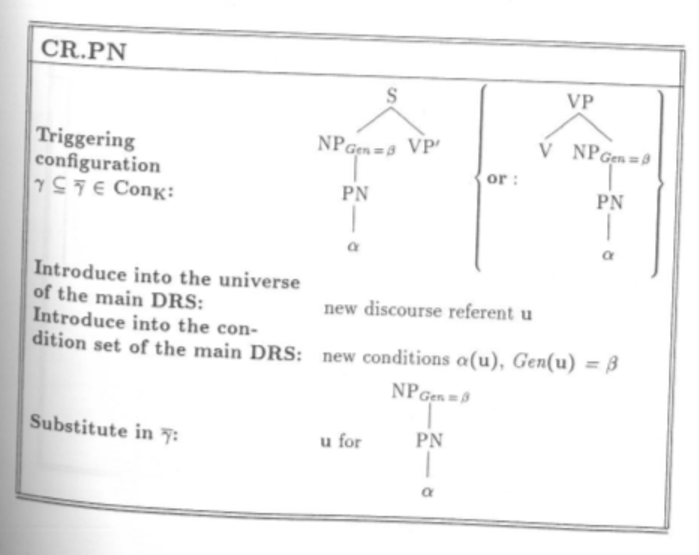
\includegraphics[width=\textwidth]{cr-pn}
\end{frame}

\begin{frame}{Adding Presuppositions}
  introduce a new abstract operation
  $$
  E_p = \{ \typedop{presuppose}{(\iota \to o)}{\iota} \}
  $$
  \vfill
  \pause
  and a corresponding open handler
  \begin{align*}
  \texttt{ACCOMODATE} &: \FF_{E_p \uplus E_f}(\alpha) \to \FF_{E_d \uplus E_f}(\alpha) \\
  \end{align*}
  \vspace{-1cm}
  \begin{align*}
    \texttt{ACCOMODATE} = \banana{\onto{\op{presuppose}}{(\lam{p k}
        {&\app{\op{introduce}}{\star}{(\lam{u}\\
        {&\app{\op{assert}}{(\ap{p}{u})}{(\lam{\_}\\
        {&\ap{k}{u}})}})}})}}
  \end{align*}
  \vfill
  \pause
  Note:
  \begin{itemize}
  \item needs slight change to $\get$
  \item supports local/intermediate accomodation also
    \begin{itemize}
    \item just add a $\op{presuppose}$ clause in $\oboxop$
    \end{itemize}
  \end{itemize}
\end{frame}

\begin{frame}{Adding Deixis}
  introduce a new abstract operation
  $$
  E_m = \{ \typedop{me}{1}{\iota} \}
  $$
  \vfill
  \pause
  and a corresponding open handler
  \begin{align*}
    \texttt{IDENTIFY} &: \iota \to \FF_{E_m \uplus E_f}(\alpha) \to \FF_{E_f}(\alpha) \\
    \texttt{IDENTIFY} &= \lam{i A}{\ap{\banana{\onto{\op{me}}{(\lam{\_ k}{\ap{k}{i}})}}}{A}}
  \end{align*}
  \vfill
  \pause
  and then use in lexical entries
  \pause

  Note:
  \begin{itemize}
  \item can also be used for time, current world and other indices
  \end{itemize}
\end{frame}

\begin{frame}{Adding Expressives}
  introduce a new abstract operation
  $$
  E_e = \{ \typedop{express}{\epsilon}{1} \}
  $$
  \vfill
  \pause
  and a corresponding open handler
  \begin{align*}
    \texttt{COLLECT} &: \FF_{E_e \uplus E_f}(\alpha) \to \FF_{E_f}(\alpha \times \epsilon) \\
  \end{align*}
  \vspace{-1cm}
  \begin{align*}
    \texttt{COLLECT} = \banana{&\onto{\op{express}}{(\lam{e k}{(\lam{(x,
            e')}{(x, e + e')}) \apr (\ap{k}{e})})}, \\
                               &\onto{\eta}{(\lam{x}{\ap{\eta}{(x, 0)}})}}
  \end{align*}
\end{frame}



\begin{frame}{Summary}
  \begin{itemize}
  \item DRT hides a programming language inside
    \pause
  \item we can characterize it in a concise signature
    \pause
  \item we can instantiate that to get continuation-based dynamic logic
    \pause
  \item we can also instantiate it in a calculus with effects and handlers
  \end{itemize}
\end{frame}

\end{document}
